% ------------------------------------------------------------------
% Aqui, o objetivo é mostrar como colocar uma imagem ou um gráfico 
% na presente monografia. tudo que faremos é usar um ambiente 
% gráfico e assim, iremos o gerar. 
%-------------------------------------------------------------------

%-------------------------------------------------------------------
% Novamente, para preenchermos o documento, usaremos o lipsum
%-------------------------------------------------------------------

\chapter{graficos}
\label{cap:graf}

\lipsum[37]

%-------------------------------------------------------------------
% O que faremos abaixo é incluir uma imagem (formato JPG, mas 
% poderia ser outro formato) no pdf. O argumento width=\textwidth 
% ajusta a largura da imagem a largura da página
%-------------------------------------------------------------------

\begin{figure}[h]
	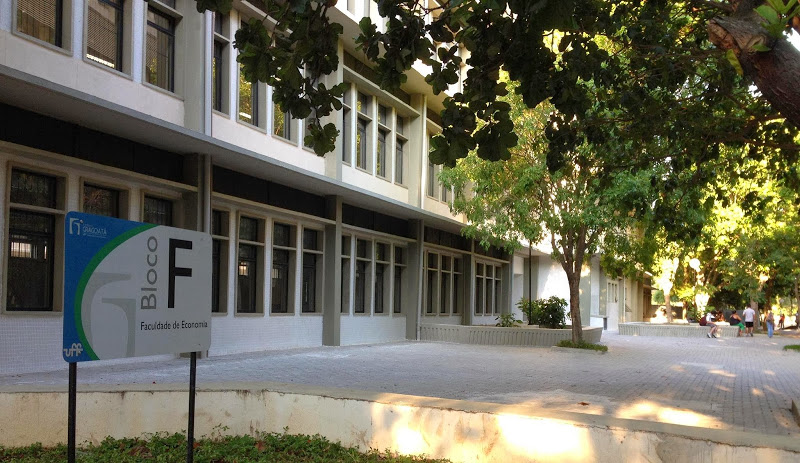
\includegraphics[width=\textwidth]{imagens/blocof.jpg}
	\caption{O Bloco F}
	\label{fig:blocof} % Aqui 'nomeamos' o gráfico
\end{figure}

%-------------------------------------------------------------------
% mais lipsum...
%-------------------------------------------------------------------

\lipsum[35-36]